% Provenance (never printed): old seconde/premiere S material on water as a
% resource (stocks and flows of the water cycle, residence times, groundwater,
% overuse as a physical fact); see sources/book2/PROVENANCE.md. Residence
% times are computed in figdata/grade-10/residence_times.py, the Aral Sea
% budget in figdata/grade-10/aral_sea.py.
\chapter{Los recursos de agua dulce}\label{ch:g10:freshwater-resources}

En 1960, el mar de Aral, en los desiertos de Asia Central, era el cuarto
lago más grande del mundo. Dos grandes ríos, alimentados por la nieve y la
lluvia de montañas lejanas, desembocaban en él; ninguno salía de él. En los
años sesenta su agua se desvió para regar el desierto. Los satélites han
observado lo que vino después: el lago se ha roto en pedazos, y la mayor parte
de su lecho es hoy tierra seca. La causa, de manera abrumadora, no fue un
cambio de clima, sino el regadío: el lago recibía mucha menos agua de la que
la evaporación le quitaba cada año. Este capítulo cuenta el agua de la Tierra, dónde
se almacena y a qué velocidad se mueve, y muestra que un recurso de agua es
ante todo un \omterm{def:g10:freshwater-resources:stock}{flujo}: cuando se saca de un depósito más agua de la que entra en
él, el depósito se vacía, a un ritmo que un simple balance permite prever.
% ledger: nasa:aral, gaybullaev:aral-1960, micklin:aral

\begin{omfigure}
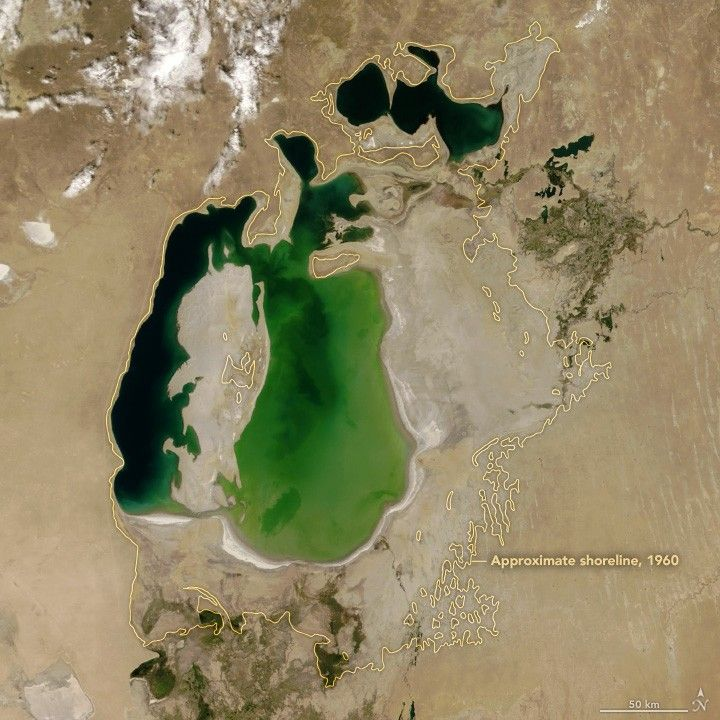
\includegraphics[width=0.47\linewidth]{images/book2/g10-nasa-aral-2000.jpg}\hspace{0.03\linewidth}%
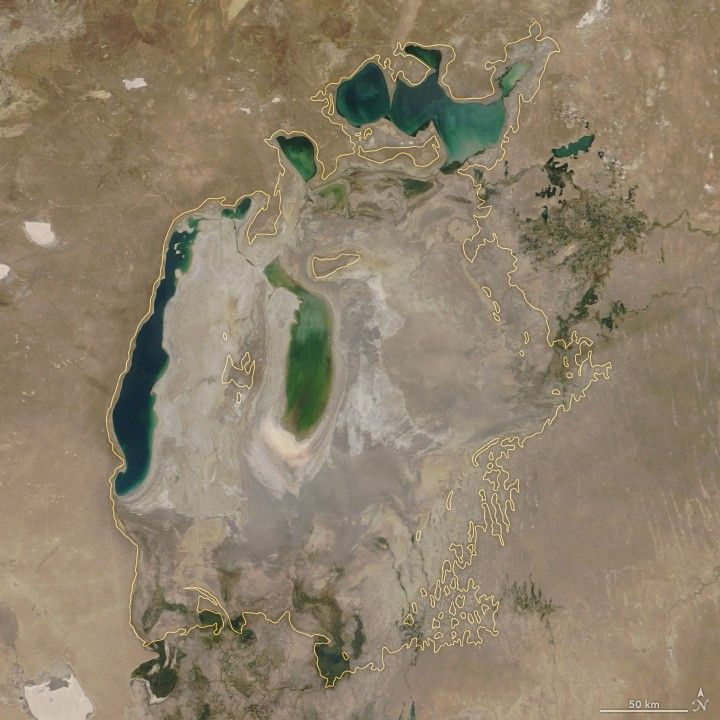
\includegraphics[width=0.47\linewidth]{images/book2/g10-nasa-aral-2018.jpg}

{\small El mar de Aral visto por el instrumento MODIS del satélite Terra de
la NASA en agosto de 2000 (izquierda) y en agosto de 2018 (derecha); la línea
amarilla es la orilla aproximada de 1960. La barra de escala mide
\qty{50}{km}. Imágenes: NASA Earth Observatory.}
\end{omfigure}

\begin{recall}
El ciclo del agua mueve el agua entre el océano, el aire y las tierras
emergidas: evaporación, condensación en nubes, precipitación, escorrentía; la
masa total de agua se conserva (los libros de física). Las rocas con poros
comunicados son permeables; por debajo del nivel freático sus poros están
llenos de agua, y una capa que contiene y deja pasar agua suficiente para
alimentar pozos es un acuífero (Libro 1, año 6). La mayor parte del agua de
la Tierra es agua salada (Libro 1, año 2). Un río se lleva el agua de su
\omterm{def:g10:drainage-basins:drainage-basin}{cuenca hidrográfica}; su \omterm{def:g10:drainage-basins:discharge}{caudal} es un volumen por segundo (el
\cref{ch:g10:drainage-basins}).
\end{recall}

\section{Dónde está el agua}

La Tierra contiene unos 1390 millones de kilómetros cúbicos de agua. Casi
toda está en el océano; solo el \qty{2.5}{\percent} es dulce. Y la mayor parte
de esa agua dulce está fuera de nuestro alcance: más de dos tercios están
helados en los casquetes de hielo y los glaciares, y casi un tercio está bajo
tierra.
% ledger: usgs:water-stocks

\begin{center}
\small
\begin{tabular}{|l|r|r|}
\hline
\textbf{depósito} & \textbf{volumen (\unit{km^3})} & \textbf{parte del agua dulce} \\ \hline
océanos, mares y bahías & \num{1338000000} & (salada) \\ \hline
casquetes de hielo, glaciares y nieves perpetuas & \num{24064000} & \qty{68.7}{\percent} \\ \hline
agua subterránea dulce & \num{10530000} & \qty{30.1}{\percent} \\ \hline
hielo del suelo y permafrost & \num{300000} & \qty{0.86}{\percent} \\ \hline
lagos de agua dulce & \num{91000} & \qty{0.26}{\percent} \\ \hline
humedad del suelo & \num{16500} & \qty{0.05}{\percent} \\ \hline
atmósfera & \num{12900} & \qty{0.04}{\percent} \\ \hline
ríos & \num{2120} & \qty{0.006}{\percent} \\ \hline
\end{tabular}

{\small Una estimación del agua del mundo, según Shiklomanov (1993), tomada
del U.S. Geological Survey. Se excluyen el agua subterránea salina
(\num{12870000}~\unit{km^3}) y los lagos salados.}
\end{center}
% ledger: usgs:water-stocks

Los ríos y los lagos de agua dulce, de los que la gente saca la mayor parte
del agua que usa, contienen juntos menos de una centésima parte del uno por
ciento de toda el agua. Y sin embargo los ríos nunca se secan por mucho
tiempo: no son una \omterm{def:g10:freshwater-resources:stock}{reserva}, sino un \omterm{def:g10:freshwater-resources:stock}{flujo}, que cada lluvia vuelve a llenar.

\section{Reservas y flujos}

\begin{definition}[Reserva; flujo]\label{def:g10:freshwater-resources:stock}
En un balance de agua, una \emph{reserva}\index{reserva (de agua)} es la
cantidad de agua contenida en un depósito --- el océano, el aire, el hielo,
un acuífero, un lago --- en un momento dado, expresada como volumen o como
masa. Un \emph{flujo}\index{flujo (de agua)} es la cantidad que pasa de un depósito a otro por unidad
de tiempo, por ejemplo en kilómetros cúbicos por año.
\end{definition}

Una \omterm{def:g10:freshwater-resources:stock}{reserva} solo cambia a través de sus \omterm{def:g10:freshwater-resources:stock}{flujos}: lo que entra menos lo que
sale. Cuando los dos son iguales, la \omterm{def:g10:freshwater-resources:stock}{reserva} está en \emph{estado
estacionario}: se mantiene igual aunque su agua se esté renovando sin cesar.

\begin{omfigure}
\begin{tikzpicture}[font=\footnotesize, >={Stealth[length=6pt]}]
  % ocean, land, atmosphere
  \fill[omSea] (0,0) rectangle (6.4,1.6);
  \fill[omLithAlluv] (6.4,0) -- (6.4,1.6) -- (8.2,2.1) -- (10.4,2.6) -- (12,2.9) -- (12,0) -- cycle;
  \fill[omLithSand!60] (6.4,0) -- (12,0) -- (12,1.0) -- (6.4,0.7) -- cycle;
  \draw[black!50] (6.4,1.6) -- (8.2,2.1) -- (10.4,2.6) -- (12,2.9);
  \fill[omIce] (10.6,2.65) -- (11.3,3.35) -- (12,2.9) -- cycle;
  \node[align=center] at (3.2,0.75) {\textbf{océano}\\\num{1335040}};
  \node[align=center] at (9.3,1.35) {humedad del suelo 122\\lagos y ríos 178};
  \node[align=center] at (9.3,0.35) {agua subterránea \num{15300}};
  \node[align=center] at (11.2,2.25) {hielo\\\num{26350}};
  % atmosphere
  \draw[black!30, rounded corners=8pt, fill=omWxCloud] (1.0,4.6) rectangle (11.0,5.6);
  \node[align=center] at (6.0,5.1) {\textbf{atmósfera} 12.7};
  % fluxes
  \draw[->, omProp, line width=1.4pt] (1.4,1.7) -- node[left, align=right] {evaporación\\413} (1.4,4.5);
  \draw[->, omWxRain, line width=1.4pt] (4.4,4.5) -- node[pos=0.3, right, align=left] {precipitación\\373} (4.4,1.7);
  \draw[->, omWxRain, line width=1.4pt] (7.6,4.5) -- node[pos=0.7, left, align=right] {precipitación\\113} (7.6,2.05);
  \draw[->, omProp, line width=1.4pt] (10.0,2.6) -- node[right, align=left] {evaporación y\\transpiración 73} (10.0,4.5);
  \draw[->, black!60, line width=1.2pt] (4.9,5.85) -- node[above] {vapor de agua llevado sobre las tierras: 40} (7.4,5.85);
  \draw[->, omRiver, line width=1.4pt] (7.6,1.2) -- node[above, inner sep=2pt] {escorrentía 40} (6.0,1.2);
\end{tikzpicture}

{\small El ciclo global del agua en los años noventa (esquema, sin escala).
\omterm{def:g10:freshwater-resources:stock}{Reservas} en miles de \unit{km^3}; \omterm{def:g10:freshwater-resources:stock}{flujos} en miles de \unit{km^3} por año.
Según Trenberth y colaboradores (2007). Las estimaciones de las \omterm{def:g10:freshwater-resources:stock}{reservas}
difieren de un estudio a otro: compara aquí el agua subterránea y el hielo
con la tabla anterior.}
\end{omfigure}
% ledger: trenberth:water-cycle

El ciclo está equilibrado. Cada año, el océano pierde \num{413000}~\unit{km^3}
por evaporación y recupera \num{373000} en forma de lluvia y nieve y
\num{40000} de los ríos. El aire recibe $413\,000 + 73\,000 = \num{486000}$~\unit{km^3}
y devuelve $373\,000 + 113\,000$, lo mismo. Las tierras emergidas reciben
\num{113000}~\unit{km^3} de precipitación; \num{73000} vuelven al aire por
evaporación y a través de las hojas de las plantas, y los \num{40000}
restantes van a parar al mar, por los ríos y bajo tierra.
% ledger: trenberth:water-cycle

\begin{definition}[Agua dulce renovable]\label{def:g10:freshwater-resources:renewable}
El \emph{agua dulce renovable}\index{agua dulce renovable} de una región es el
\omterm{def:g10:freshwater-resources:stock}{flujo} de agua dulce que la precipitación renueva cada año y que la atraviesa
como escorrentía en los ríos y como agua subterránea. Es un \omterm{def:g10:freshwater-resources:stock}{flujo}, en
kilómetros cúbicos por año, no una \omterm{def:g10:freshwater-resources:stock}{reserva}.
\end{definition}

Para el conjunto de las tierras emergidas, son los \num{40000}~\unit{km^3} que
llegan al mar cada año. Una región puede usar su agua renovable año tras año
sin quedarse corta. Lo que tome por encima de ella solo puede salir de una
\omterm{def:g10:freshwater-resources:stock}{reserva}, que entonces mengua.

\section{El tiempo de residencia}

¿Cuánto tiempo pasa una molécula de agua en un depósito? Algunas se van
enseguida, otras se quedan mucho más; pero, en promedio, la respuesta se
deduce solo de la \omterm{def:g10:freshwater-resources:stock}{reserva} y del \omterm{def:g10:freshwater-resources:stock}{flujo}.

\begin{definition}[Tiempo de residencia]\label{def:g10:freshwater-resources:residence-time}
El \emph{tiempo de residencia}\index{tiempo de residencia} del agua en un
depósito es el tiempo medio que el agua pasa en él entre su entrada y su
salida.
\end{definition}

\begin{proposition}[Tiempo de residencia, reserva y flujo]\label{prop:g10:freshwater-resources:residence}
Para un depósito en estado estacionario, que contiene una \omterm{def:g10:freshwater-resources:stock}{reserva} $S$ y es
atravesado por un \omterm{def:g10:freshwater-resources:stock}{flujo} $F$ (de entrada y de salida), el \omterm{def:g10:freshwater-resources:residence-time}{tiempo de residencia}
es
\[
T = \frac{S}{F}.
\]
\end{proposition}

\begin{proof}
En estado estacionario, cada año entra un volumen $F$ y sale un volumen $F$,
mientras la \omterm{def:g10:freshwater-resources:stock}{reserva} sigue siendo $S$. Al cabo de un tiempo $S/F$, ha entrado un
volumen $F \times S/F = S$: tanto como contiene todo el depósito. En promedio,
el agua presente al principio ha sido entonces sustituida, así que el agua
pasa $S/F$ en el depósito.
\end{proof}

\begin{example}[El agua del aire]\label{ex:g10:freshwater-resources:atmosphere}
La atmósfera contiene \num{12700}~\unit{km^3} de agua, y cada año caen de ella
\num{486000}~\unit{km^3} en forma de lluvia y nieve. Su \omterm{def:g10:freshwater-resources:residence-time}{tiempo de residencia}
es de $12\,700/486\,000 \approx \num{0.026}$ años, unos \num{9.5} días: el
agua del aire se renueva cada semana o dos. Una nube que llueve hoy está hecha
de agua que salió del océano o del suelo hace unos pocos días.
\end{example}
% ledger: trenberth:water-cycle (t_atmosphere_days 9.5 in figdata/grade-10/residence_times.py)

El mismo cálculo da unos \num{19} días para el agua de los cauces de los ríos
($2120$~\unit{km^3} recorridos por \num{40000}~\unit{km^3} al año), unos
pocos años para los lagos y los ríos juntos, y unos \num{3200} años para el
océano ($1\,335\,040/413$ miles de~\unit{km^3}). El agua subterránea puede ser
más lenta todavía: el agua más profunda de algunos acuíferos tiene cientos de
miles de años.
% ledger: trenberth:water-cycle, usgs:water-stocks, sturchio:nubian-age

\begin{omfigure}
\begin{tikzpicture}
\begin{axis}[omrecord, xbar, xmode=log, log origin=infty, width=0.74\linewidth, height=5.6cm,
  xmin=1, xmax=1e9, ymin=-0.6, ymax=4.6, bar width=11pt,
  ytick={0,1,2,3,4}, yticklabels={atmósfera, ríos, {lagos y ríos}, océano, {agua subterránea profunda (edad)}},
  xtick={1,30.44,365.25,36525,3652500,365250000}, xticklabels={1 día, 1 mes, 1 año, 100 años, \num{10000} años, 1 millón de años},
  xticklabel style={font=\scriptsize, rotate=25, anchor=north east}, yticklabel style={font=\small},
  xlabel={tiempo de residencia (escala logarítmica)}, label style={font=\small}, xmajorgrids]
\addplot[fill=omDef!45, draw=omDef!80!black] table[x=days, y=idx] {figdata/out/grade-10-residence_times-times.dat};
\draw[fill=omProp!45, draw=omProp!80!black] (axis cs:73050000,3.75) rectangle (axis cs:365250000,4.25);
\node[anchor=west, font=\scriptsize] at (axis cs:9.5,0) {\num{9.5} días};
\node[anchor=west, font=\scriptsize] at (axis cs:19.4,1) {\num{19} días};
\node[anchor=west, font=\scriptsize] at (axis cs:1625,2) {\num{4.5} años};
\node[anchor=west, font=\scriptsize] at (axis cs:1180690,3) {\num{3200} años};
\node[anchor=east, font=\scriptsize] at (axis cs:73050000,4) {de \num{200000} a 1 millón de años};
\end{axis}
\end{tikzpicture}

{\small \omterm{def:g10:freshwater-resources:residence-time}{Tiempos de residencia} del agua, calculados como \omterm{def:g10:freshwater-resources:stock}{reserva} dividida entre
\omterm{def:g10:freshwater-resources:stock}{flujo} a partir del ciclo global del agua (azul), y edad medida del agua
subterránea profunda bajo el este del Sahara (naranja). Eje logarítmico: a
partir de un año, cada escalón marcado multiplica por cien. Datos:
Trenberth y colaboradores (2007); U.S. Geological Survey; Sturchio y
colaboradores (2004).}
\end{omfigure}
% values computed in figdata/grade-10/residence_times.py

El \omterm{def:g10:freshwater-resources:residence-time}{tiempo de residencia} mide la rapidez con que se recupera un depósito. El
agua tomada de un río se repone en días; un lago contaminado o vaciado tarda
años; el agua subterránea que tardó miles de años en reunirse no se renueva
en absoluto a la escala de una vida humana.

\begin{method}[Un balance de agua]\label{met:g10:freshwater-resources:budget}
\begin{enumerate}
  \item Elige el depósito: un lago, un acuífero, una cuenca, el aire.
  \item Haz la lista de todos los \omterm{def:g10:freshwater-resources:stock}{flujos} que entran en él (ríos, lluvia,
        infiltración) y que salen de él (ríos, evaporación, bombeo), en la
        misma unidad.
  \item La variación anual de la \omterm{def:g10:freshwater-resources:stock}{reserva} es la suma de las entradas menos la
        suma de las salidas.
  \item Si la \omterm{def:g10:freshwater-resources:stock}{reserva} no cambia, las entradas igualan a las salidas, y el
        \omterm{def:g10:freshwater-resources:residence-time}{tiempo de residencia} es la \omterm{def:g10:freshwater-resources:stock}{reserva} dividida entre cualquiera de ellas.
\end{enumerate}
\end{method}

\section{Los acuíferos como depósitos}

La lluvia que se infiltra en el suelo y llega al nivel freático
\emph{recarga} el acuífero de debajo. El agua avanza luego despacio por los
poros de la roca, hacia manantiales, ríos o el mar. Donde una capa permeable
se hunde bajo una capa impermeable, como la arcilla, su agua queda
\emph{confinada}: solo se alimenta donde la capa aflora en superficie, lo que
puede ocurrir muy lejos.

\begin{omfigure}
\begin{tikzpicture}[font=\footnotesize, >={Stealth[length=5pt]}]
  % layers dipping to the right
  \fill[lith shale] (0,0) -- (12,0) -- (12,0.8) -- (0,2.4) -- cycle;
  \fill[lith sandstone] (0,2.4) -- (12,0.8) -- (12,2.2) -- (2.2,3.5) -- (0,3.8) -- cycle;
  \fill[lith shale] (2.2,3.5) -- (12,2.2) -- (12,3.4) -- (3.6,3.9) -- cycle;
  % ground surface
  \draw[line width=0.8pt, brown!60!black] (0,3.8) -- (1.2,4.0) -- (2.2,3.9) -- (3.6,3.9) -- (6,3.6) -- (9,3.5) -- (12,3.4);
  \fill[omLithAlluv] (0,3.8) -- (1.2,4.0) -- (2.2,3.9) -- (2.2,3.5) -- (0,3.8) -- cycle;
  \fill[omLithAlluv] (2.2,3.9) -- (3.6,3.9) -- (2.2,3.5) -- cycle;
  \fill[omLithAlluv] (3.6,3.9) -- (6,3.6) -- (9,3.5) -- (12,3.4) -- (3.6,3.9) -- cycle;
  % water table in the unconfined part
  \draw[omDef, line width=1pt, dashed] (0,3.3) .. controls (1.0,3.35) and (1.8,3.2) .. (2.6,3.45);
  \node[anchor=south west, text=omDef, fill=white, fill opacity=0.8, text opacity=1, inner sep=1pt] at (0.05,2.75) {nivel freático};
  % rain and recharge
  \foreach \x in {0.35,0.65,0.95,1.25} \draw[omWxRain, thick] (\x,4.9) -- (\x-0.15,4.4);
  \node[anchor=south, text=omWxRain] at (0.7,4.95) {lluvia: recarga};
  % flow arrows in the aquifer
  \draw[->, omDef, line width=1.1pt] (2.0,2.85) -- (4.4,2.55);
  \draw[->, omDef, line width=1.1pt] (5.4,2.4) -- (7.8,2.1);
  \draw[->, omDef, line width=1.1pt] (8.8,1.95) -- (11.2,1.65);
  % wells
  \draw[black!70, line width=1.6pt] (1.95,3.95) -- (1.95,2.9);
  \node[anchor=south] at (1.95,4.0) {pozo};
  \draw[black!70, line width=1.6pt] (7.0,3.55) -- (7.0,1.9);
  \node[anchor=south] at (7.0,3.6) {pozo};
  % labels
  \node[align=center, fill=white, fill opacity=0.85, text opacity=1, inner sep=1.5pt] at (1.5,0.8) {arcilla impermeable};
  \node[align=center, fill=white, fill opacity=0.85, text opacity=1, inner sep=1.5pt] at (8.6,2.95) {arcilla impermeable};
  \node[anchor=north, align=center] at (1.6,-0.1) {acuífero libre:\\zona de recarga};
  \node[anchor=north, align=center] at (6.4,-0.1) {acuífero confinado};
  \node[anchor=north, align=center] at (10.6,-0.1) {agua antigua, lejos de\\la zona de recarga};
\end{tikzpicture}

{\small Un acuífero en una arenisca permeable (esquema). La lluvia lo recarga
donde aflora en superficie; allí el nivel freático puede subir y bajar
libremente. Más lejos, bajo la arcilla, el acuífero está confinado, y su agua
avanza despacio a lo largo de la capa: cuanto más lejos de la zona de
recarga, más antigua es el agua.}
\end{omfigure}

\begin{definition}[Agua subterránea fósil]\label{def:g10:freshwater-resources:fossil-groundwater}
El \emph{agua subterránea fósil}\index{agua subterranea fosil@agua subterránea fósil}
es el agua subterránea que entró en su acuífero hace mucho tiempo, a menudo
con un clima más húmedo, y que la recarga actual no renueva a la escala de
las vidas humanas.
\end{definition}

Bajo el este del Sahara se extiende un enorme acuífero de arenisca. Su agua
más profunda, datada por la desintegración de una forma radiactiva rara del
criptón, tiene entre \num{200000} años y un millón de años. Llegó despacio
desde una zona de recarga del suroeste de Egipto, y su química muestra que
cayó en forma de lluvia durante periodos húmedos de las glaciaciones, cuando
el aire húmedo del Atlántico llegaba a la región. Bombeada hoy, esta agua es
una \omterm{def:g10:freshwater-resources:stock}{reserva} que se agota, no un \omterm{def:g10:freshwater-resources:stock}{flujo}.
% ledger: sturchio:nubian-age

Cuando el bombeo supera la recarga, el nivel freático baja. En las Altas
Llanuras del centro de Estados Unidos, el acuífero que hay bajo unas
\num{175000} millas cuadradas (\qty{453000}{km^2}) se bombea para el regadío
desde hacia 1950. En 2015 su nivel de agua había bajado \qty{4.8}{m} de media,
y hasta \qty{71}{m} (234 pies) en algunos pozos; el acuífero había perdido
unos \num{273} millones de acres-pie de agua, unos \qty{340}{km^3}.
% ledger: mcguire:high-plains (1 acre-foot = 1233.5 m3)

\begin{omfigure}
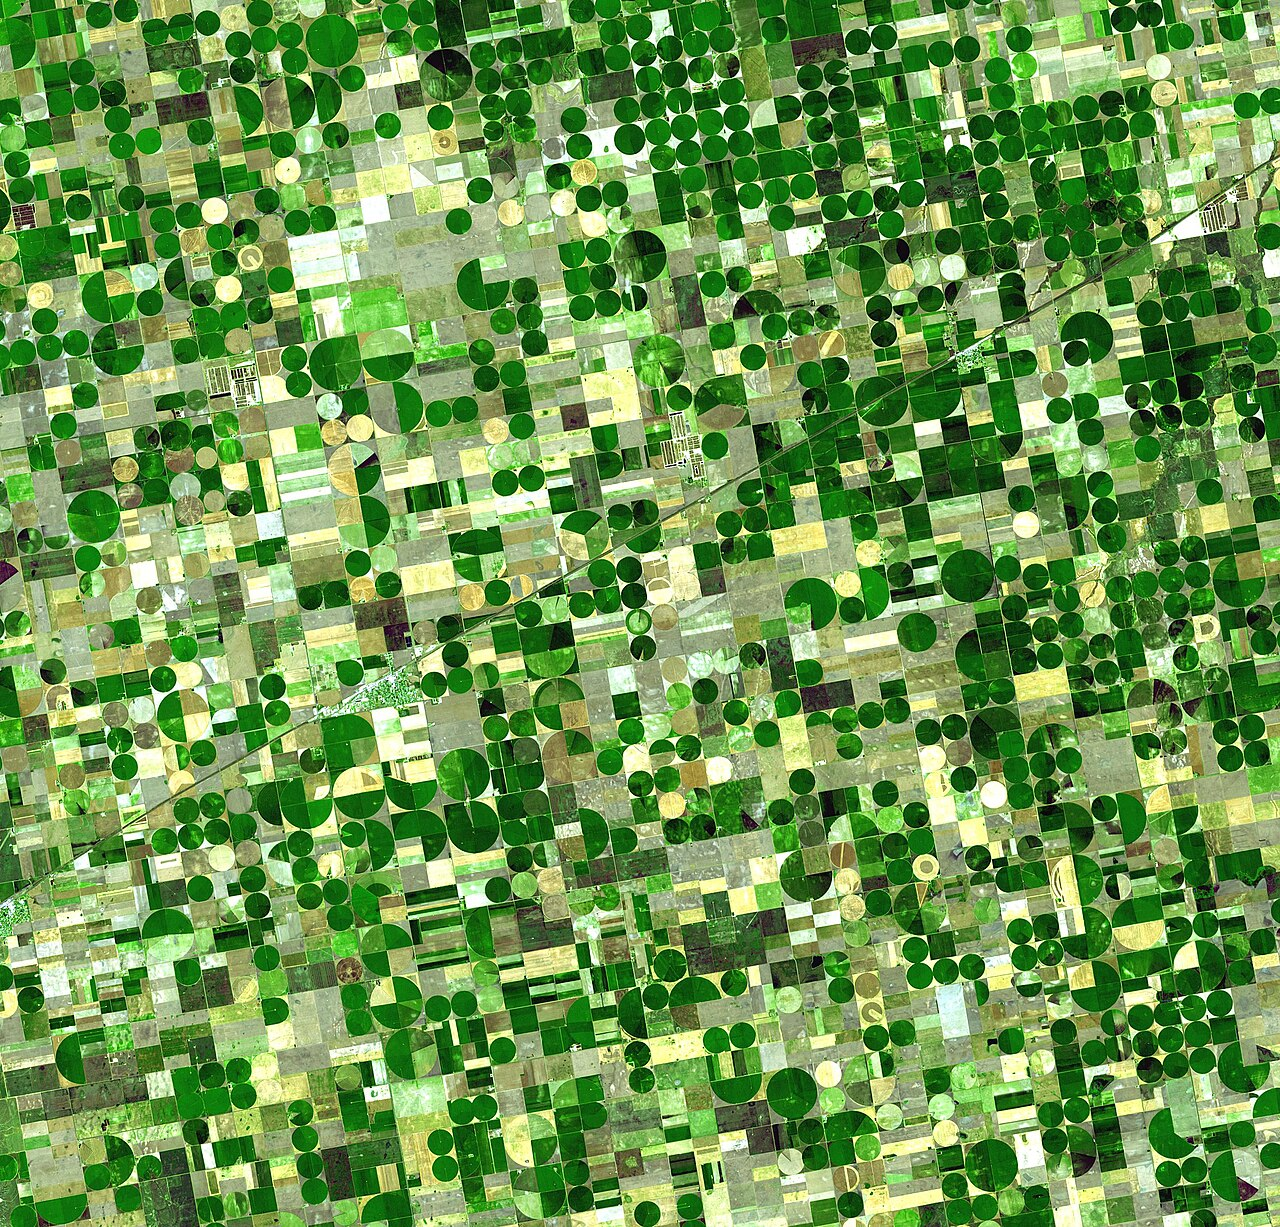
\includegraphics[width=0.5\linewidth]{images/book2/g10-nasa-kansas-center-pivot.jpg}

{\small Campos de regadío cerca de Sublette, en Kansas, vistos por el
instrumento ASTER del satélite Terra de la NASA en junio de 2001 (unos
\qty{37}{km} de lado a lado). Cada círculo es un campo regado por un largo
brazo aspersor que gira alrededor de su centro; los círculos miden \num{800}
y \qty{1600}{m} de diámetro. Imagen: NASA (dominio público).}
\end{omfigure}

El agua subterránea no se ve desde el espacio, pero se puede pesar: dos
satélites que vuelan uno detrás del otro notan los ligeros cambios de la
atracción de la Tierra causados por la masa de agua que va y viene debajo de
ellos, y cartografían dónde sube y dónde baja de un mes a otro la \omterm{def:g10:freshwater-resources:stock}{reserva} de
agua en las tierras emergidas.

\begin{omfigure}
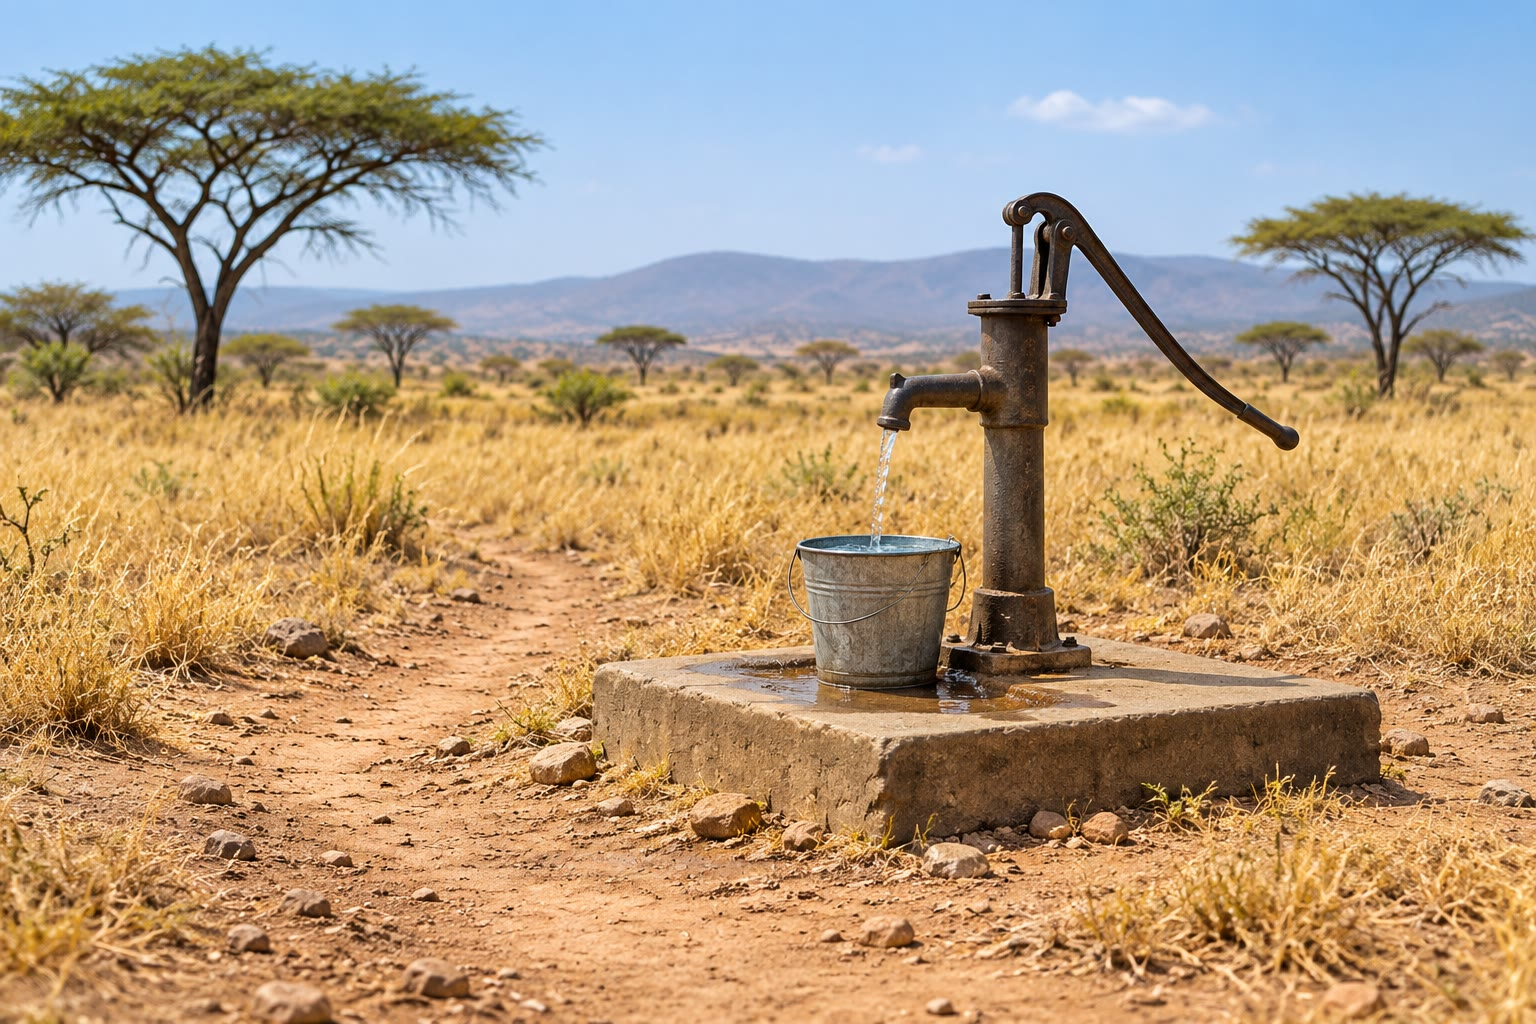
\includegraphics[width=0.55\linewidth]{images/book2/ai/g10-hand-pump-well.jpg}

{\small Una bomba de mano sobre un pozo en un paisaje seco: el agua que se saca
aquí viene del subsuelo, fuera del alcance de la estación seca.}
\end{omfigure}

\section{La sobreexplotación como hecho físico}

El mar de Aral no tiene desagüe: el agua de sus dos ríos, el Amu Daria y el
Sir Daria, solo sale por evaporación. En 1960 cubría \qty{68000}{km^2},
contenía \qty{1093}{km^3} y su agua tenía \qty{10}{g} de sal por litro. Ese
año, la evaporación le quitó \qty{71.1}{km^3}, y la lluvia sobre el lago le
aportó \qty{9.4}{km^3}: para mantener su nivel, el lago necesitaba recibir de
sus ríos $71.1 - 9.4 = \qty{61.7}{km^3}$ al año.
% ledger: gaybullaev:aral-1960, gaybullaev:aral-table

A partir de los años sesenta, los ríos se desviaron para regar el desierto, y
casi nada de su agua llegaba al lago: en los años setenta y ochenta, a menudo
menos de \qty{2}{km^3} al año. La evaporación continuó, y el lago
empezó a encogerse. Su balance marca la velocidad. La evaporación se lleva una
capa de agua cuyo espesor depende del clima, aquí de alrededor de un metro al
año ($71.1/68\,000 \approx \qty{0.00105}{km}$). Si los aportes se detienen,
el nivel baja más o menos eso cada año, menos la lluvia. A medida que el lago
se encoge, su superficie, y con ella su evaporación, también disminuyen, y la
bajada se frena; pero no se detiene hasta que los aportes y la evaporación
vuelven a equilibrarse.
% ledger: gaybullaev:aral-table (values computed in figdata/grade-10/aral_sea.py)

\begin{omfigure}
\begin{tikzpicture}
\begin{axis}[omrecord, name=vol, width=0.46\linewidth, height=5.4cm, xmin=1955, xmax=2012, ymin=0, ymax=1200,
  xtick={1960,1980,2000}, xticklabel style={/pgf/number format/1000 sep={}}, scaled y ticks=false,
  ylabel={volumen (\unit{km^3})}, xlabel={año}, tick label style={font=\small}, label style={font=\small},
  title={\small volumen de agua}]
\addplot[omDef, line width=1pt, mark=*, mark size=1.3pt] table[x=year, y=volume] {figdata/out/grade-10-aral_sea-record.dat};
\end{axis}
\begin{axis}[omrecord, at={(vol.east)}, anchor=west, xshift=1.4cm, width=0.46\linewidth, height=5.4cm,
  xmin=1955, xmax=2012, ymin=0, ymax=140, xtick={1960,1980,2000},
  xticklabel style={/pgf/number format/1000 sep={}},
  ylabel={salinidad (\unit{g/L})}, xlabel={año}, tick label style={font=\small}, label style={font=\small},
  title={\small salinidad}]
\addplot[omProp, line width=1pt, mark=*, mark size=1.3pt] table[x=year, y=salinity] {figdata/out/grade-10-aral_sea-record.dat};
\end{axis}
\end{tikzpicture}

{\small El mar de Aral de 1960 a 2010: el volumen de su agua bajó a la décima
parte, mientras que la sal que dejaba la evaporación se concentró trece veces
más. Datos: Gaybullaev y colaboradores (2012).}
\end{omfigure}
% ledger: gaybullaev:aral-table

En 2010 el lago contenía \qty{98}{km^3}, la décima parte de su volumen de
1960, sobre \qty{14280}{km^2}; su salinidad había llegado a \qty{130}{g/L},
mucho más salada que el océano. Su nivel había bajado más de \qty{20}{m}. Del
lecho seco se levanta un polvo salado. La causa no es ningún misterio: se
cortaron los aportes del lago, pero no su evaporación.
% ledger: gaybullaev:aral-table, gaybullaev:aral-1960, micklin:aral, nasa:aral

\section{Ejercicios}

\begin{exercise}[$\star$]\label{exo:g10:freshwater-resources:1}
Define una \omterm{def:g10:freshwater-resources:stock}{reserva}, un \omterm{def:g10:freshwater-resources:stock}{flujo} y un \omterm{def:g10:freshwater-resources:residence-time}{tiempo de residencia}, y da las unidades de
cada uno.
\end{exercise}

\begin{exercise}[$\star$]\label{exo:g10:freshwater-resources:2}
Con la tabla del agua del mundo: ¿qué parte de toda el agua es dulce? Del
agua dulce, ¿qué partes están heladas y bajo tierra? ¿Qué depósito contiene
menos?
\end{exercise}

\begin{exercise}[$\star$]\label{exo:g10:freshwater-resources:3}
Define el \omterm{def:g10:freshwater-resources:renewable}{agua dulce renovable} y el \omterm{def:g10:freshwater-resources:fossil-groundwater}{agua subterránea fósil}. ¿Por qué la
primera es un \omterm{def:g10:freshwater-resources:stock}{flujo} y la segunda una \omterm{def:g10:freshwater-resources:stock}{reserva}?
\end{exercise}

\begin{exercise}[$\star$]\label{exo:g10:freshwater-resources:4}
¿Cuántas veces más agua contienen los lagos de agua dulce del mundo
(\num{91000}~\unit{km^3}) que sus ríos (\num{2120}~\unit{km^3})?
\end{exercise}

\begin{exercise}[$\star$]\label{exo:g10:freshwater-resources:5}
En la gráfica de los \omterm{def:g10:freshwater-resources:residence-time}{tiempos de residencia}, ¿qué depósito renueva su agua más
deprisa, y cuál más despacio? ¿Cuántas veces más tiempo pasa el agua en el
océano que en el aire?
\end{exercise}

\begin{exercise}[$\star\star$]\label{exo:g10:freshwater-resources:6}
La atmósfera contiene \num{12700}~\unit{km^3} de agua. Calcula su \omterm{def:g10:freshwater-resources:residence-time}{tiempo de
residencia} a partir de la evaporación que entra en ella (\num{413000} desde el
océano y \num{73000}~\unit{km^3} desde las tierras emergidas cada año), y
comprueba que coincide con el \omterm{def:g10:freshwater-resources:residence-time}{tiempo de residencia} calculado a partir de la
precipitación que sale de ella.
\end{exercise}

\begin{exercise}[$\star\star$]\label{exo:g10:freshwater-resources:7}
El océano contiene \num{1335040} miles de~\unit{km^3} y pierde \num{413}
miles de~\unit{km^3} al año por evaporación. Calcula su \omterm{def:g10:freshwater-resources:residence-time}{tiempo de residencia}.
¿Por qué es el mismo si se calcula con lo que entra en él?
\end{exercise}

\begin{exercise}[$\star\star$]\label{exo:g10:freshwater-resources:8}
Con los \omterm{def:g10:freshwater-resources:stock}{flujos} del ciclo global del agua, escribe el balance de las tierras
emergidas: lo que cae sobre ellas, lo que vuelve al aire y lo que se escurre.
¿Qué parte de la lluvia que cae sobre las tierras vuelve al aire?
\end{exercise}

\begin{exercise}[$\star\star$]\label{exo:g10:freshwater-resources:9}
El acuífero de las Altas Llanuras perdió unos \num{273.2} millones de
acres-pie de agua desde hacia 1950 hasta 2015 (\num{1}~acre-pie =
\qty{1233.5}{m^3}). Convierte este volumen a \unit{km^3} y compáralo con el
volumen del mar de Aral en 1987 (\qty{345.6}{km^3}).
\end{exercise}

\begin{exercise}[$\star\star$]\label{exo:g10:freshwater-resources:10}
El nivel medio del agua del acuífero de las Altas Llanuras bajó \num{15.8}
pies desde hacia 1950 hasta 2015 (\num{1}~pie = \qty{0.3048}{m}). ¿Cuánto es
eso en metros, y en centímetros por año?
\end{exercise}

\begin{exercise}[$\star\star$]\label{exo:g10:freshwater-resources:11}
Un acuífero contiene \qty{2}{km^3} de agua y recibe una recarga de
\qty{0.01}{km^3} al año. ¿Cuál es el \omterm{def:g10:freshwater-resources:residence-time}{tiempo de residencia} de su agua? Ahora
unos pozos bombean de él \qty{0.05}{km^3} al año. Supón que la recarga
continúa y que los pozos son ahora la única salida del agua: ¿cuánto tiempo
durará?
\end{exercise}

\begin{exercise}[$\star\star\star$]\label{exo:g10:freshwater-resources:12}
Calcula el \omterm{def:g10:freshwater-resources:residence-time}{tiempo de residencia} del agua del mar de Aral en 1960
(\qty{1093}{km^3}, evaporación de \qty{71.1}{km^3} al año) y en 2010
(\qty{98.1}{km^3}, evaporación de \qty{11.4}{km^3} al año). ¿Por qué bajó su
evaporación?
\end{exercise}

\begin{exercise}[$\star\star\star$]\label{exo:g10:freshwater-resources:13}
Un lago sin desagüe cubre \qty{100}{km^2}. La evaporación le quita cada año
una capa de \qty{1.2}{m} de agua de su superficie, y la lluvia le añade
\qty{0.2}{m}.
\begin{enumerate}
  \item ¿Qué aporte, en \unit{km^3} al año, mantiene estable su nivel?
  \item El aporte se reduce a la mitad. ¿Cuánto baja el nivel el primer
        año?
  \item ¿Por qué se frena la bajada en los años siguientes?
\end{enumerate}
\end{exercise}

\begin{exercise}[$\star\star\star$]\label{exo:g10:freshwater-resources:14}
En un desierto, la lluvia recarga un acuífero con \qty{1}{mm} de agua al
año. El acuífero tiene \qty{100}{m} de espesor y el agua ocupa el
\qty{20}{\percent} de su volumen. ¿Cuánto tiempo tardaría la recarga en
llenarlo? Compáralo con la edad del agua profunda del acuífero del Sahara.
\end{exercise}

\begin{exercise}[$\star\star\star$]\label{exo:g10:freshwater-resources:15}
El acuífero de las Altas Llanuras cubre unos \qty{453000}{km^2} y había
perdido unos \qty{337}{km^3} de agua en 2015. ¿Qué espesor de agua,
repartida sobre todo el acuífero, es eso? Su nivel de agua bajó
\qty{4.8}{m} de media. ¿Por qué la bajada del nivel del agua es mayor que el
espesor de agua perdida?
\end{exercise}

\section{Problema: el balance del mar de Aral}

\begin{problem}[{Problema de fin de semana --- ¿a qué velocidad desaparece un lago?}]
\label{pb:g10:freshwater-resources:1}
% ledger: gaybullaev:aral-table, gaybullaev:aral-1960, micklin:aral (values computed in figdata/grade-10/aral_sea.py)
La tabla da el balance del mar de Aral para cuatro años (volúmenes en
\unit{km^3}, salinidad en gramos de sal por litro). En 1960 el lago cubría
\qty{68000}{km^2}.
\begin{center}
\small
\begin{tabular}{|c|c|c|c|c|c|}
\hline
año & aporte de los ríos & lluvia sobre el lago & evaporación & volumen & salinidad \\ \hline
1960 & 42.0 & 9.4 & 71.1 & 1093.0 & 10.0 \\ \hline
1984 & 0.3 & 3.5 & 47.9 & 502.7 & 21.9 \\ \hline
1987 & 1.0 & 6.2 & 36.8 & 345.6 & 25.0 \\ \hline
1989 & 3.1 & 5.3 & 35.3 & 327.2 & 30.0 \\ \hline
\end{tabular}

{\small Datos: Gaybullaev y colaboradores (2012).}
\end{center}

\medskip
\noindent\textbf{Parte I --- El lago en 1960.}
\begin{enumerate}
  \item ¿Cuál era la profundidad media del lago en 1960?
  \item Expresa su volumen en metros cúbicos.
  \item ¿Qué masa de sal contenía, en toneladas?
  \item ¿Cuál era el \omterm{def:g10:freshwater-resources:residence-time}{tiempo de residencia} de su agua, contado con la
        evaporación?
  \item ¿Por qué un lago sin desagüe solo puede perder agua por evaporación
        (y por infiltración)?
\end{enumerate}

\medskip
\noindent\textbf{Parte II --- Lo que necesita el lago.}
\begin{enumerate}[resume]
  \item ¿Qué espesor de agua le quitó la evaporación al lago en 1960, en
        metros?
  \item ¿Qué espesor añadió la lluvia?
  \item ¿Qué aporte de los ríos habría compensado exactamente la evaporación
        y la lluvia?
  \item Los dos ríos sacan de las montañas una media de unos \qty{79}{km^3} y
        \qty{37}{km^3} al año. ¿Qué parte de eso necesitaría el lago?
\end{enumerate}

\medskip
\noindent\textbf{Parte III --- El lago a finales de los años ochenta.}
\begin{enumerate}[resume]
  \item Escribe el balance de 1987: entradas, salidas, variación neta.
  \item Entre 1984 y 1989 el volumen bajó de \qty{502.7}{km^3} a
        \qty{327.2}{km^3}. ¿Cuál fue la bajada media por año? Compárala con
        el balance de 1987.
  \item Supón que un kilómetro cuadrado de lago pierde por evaporación tanta
        agua como en 1960. ¿Cuál era la superficie del lago en 1987?
  \item ¿Qué parte de su superficie de 1960 es eso?
  \item ¿Por qué había bajado la evaporación de \qty{71.1}{km^3} a
        \qty{36.8}{km^3}?
  \item ¿Qué parte de su volumen de 1960 conservaba todavía el lago en 1987?
\end{enumerate}

\medskip
\noindent\textbf{Parte IV --- La sal y el nivel.}
\begin{enumerate}[resume]
  \item Si toda la sal de 1960 se hubiera quedado en el agua, ¿cuál habría
        sido la salinidad en 1987?
  \item La tabla da \qty{25.0}{g/L}. ¿Qué sugiere la diferencia?
  \item Sin ningún aporte ni lluvia, ¿cuánto bajaría el nivel cada año?
  \item En 1987, ¿cuánto añadieron los ríos y la lluvia, como espesor sobre la
        superficie de la pregunta 12?
  \item ¿Cuánto bajó el nivel del mar de Aral en 1987?
\end{enumerate}
\end{problem}
